\documentclass[a4paper, 12pt]{article}

%Paragraph jumps and indentation
\setlength{\parskip}{1.5em}
\setlength{\parindent}{1.25cm}

%Border
\usepackage[left=1in, right=1in, top=1in, bottom=1in]{geometry}

%Double spacing
\usepackage{setspace}
\doublespacing

%Packages
\usepackage{amsmath}
\usepackage[dvipsnames]{xcolor}
\usepackage{mathtools}
\usepackage{amsfonts}
\usepackage{titlesec}

%Images
\usepackage{graphicx}
\graphicspath{ {./images/} }
\usepackage{wrapfig}
\usepackage{float}

%Tables
\usepackage{multirow}
\usepackage{array}
\usepackage{tabu}
\titleformat{\section}
{\normalfont\large\bfseries}{\thesection}{1em}{}
\titleformat{\subsection}
{\normalfont\large\bfseries}{\thesubsection}{1em}{}

%Equation numbering
\counterwithin{equation}{section}

%Links
\usepackage{hyperref}
\urlstyle{same}

%Diagrams
\usepackage{pgfplots}
\pgfplotsset{compat=newest}
\usetikzlibrary{positioning, arrows.meta}
\usepgfplotslibrary{fillbetween}
\usepackage{wrapfig}


\begin{document}

\begin{titlepage}
  \begin{center}
    \textbf{IB ECONOMICS} \hspace{1cm} STANDARD LEVEL\\
    \vspace*{3cm}
    \textbf{Title of the article:}
    Mozambique approves investment projects
    valued at about US\$5 billion in H1 2025\\

    \textbf{Source of the article:}
    African Mining Market\\

    \textbf{Link to the article:}
    \url{https://africanminingmarket.com/mozambique-approves-investment-projects-valued-at-about-usd5-billion-in-h1-2025}\\

    \textbf{Article publish date:}
    September 1, 2025\\

    \textbf{Article access date:} September 11, 2025\\

    \textbf{Commentary writing date:} September 11, 2025\\

    \textbf{Unit of the syllabus:}
    Macroeconomics\\

    \textbf{Key concept:}
    Intervention.\\

    \vfill
    Word count: 666
  \end{center}
\end{titlepage}

\section*{Extract}
{ \itshape
  {\large The Mozambican government has approved 115 investment projects valued at about US\$5 billion in the first half of 2025, with the potential to create 17,000 jobs. Prime Minister Benvinda Levi announced the figures on 30th August, at the closing of the 60th Maputo International Fair (FACIM).}

  The largest project is Green Energy Mozambique, a US\$3 billion industrial park in Sofala province. The complex is expected to generate 10,000 direct jobs and boost production of key materials including aluminum, steel, cement, batteries, and solar panels.

  More than 88\% of total investment was directed to Sofala, far ahead of Maputo. Foreign capital accounted for US\$3.2 billion, with contributions from investors in 25 countries. The funds mainly target industry, transport, communications, and services. Domestic investment stood at US\$144 million.

  Levi said the results show the Mozambican economy is rebounding after climate shocks and post-election tensions, with the private sector driving growth. She also highlighted the launch of a US\$250 million mutual guarantee fund during the fair to support recovery and expand private sector participation.

  These achievements align with the country's strategy to strengthen investor appeal. In recent years, Mozambique has pursued reforms to attract capital, including the creation of the Investment and Export Promotion Agency (APIEX) and the adoption of a new investment law in 2023. The country now offers tax and customs incentives, along with special economic zones in agriculture, aquaculture, and less-developed regions.

  According to UNCTAD, Mozambique ranked fourth in Africa for foreign direct investment inflows in 2024, reaching US\$3.55 billion, up from US\$2.5 billion in 2023, when it placed sixth.

}

\newpage
\section*{Commentary}

In summary, Mozambique has approved major new investment projects worth about US\$5 billion, mostly foreign-funded and centered in Sofala, including a large green energy park producing important commodities.
The initiatives are expected to create jobs and support the country's economic recovery after recent shocks, with reforms and incentives aimed at strengthening investor confidence.
This commentary will discuss how \textbf{intervention} by the government through this form of fiscal policy achieves its effects on increasing economic growth and decreasing unemployment.
The analysis shall be done with respect to the Keynesian model of aggregate demand and supply.

\begin{wrapfigure}{L}{0.5\textwidth}
  \begin{center}
    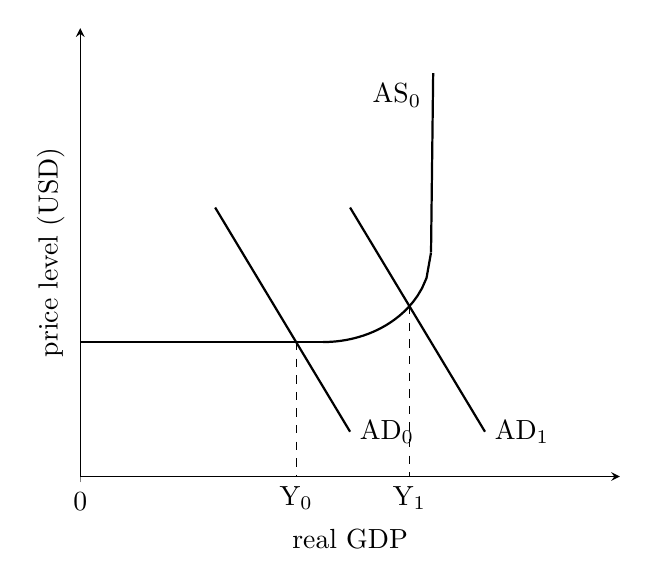
\begin{tikzpicture}[scale=1]
      \begin{axis}[
          axis lines=left,
          xlabel={real GDP},
          ylabel={price level (USD)},
          xmin=0, xmax=1,
          ymin=0, ymax=1,
          xtick={0}, ytick={\empty},
          clip=false
        ]

        \addplot[thick, domain=0:0.45] {0.3};
        \addplot[thick, domain=0.45:0.65] {0.5 - sqrt(1/25 - (x-0.45)^2)};
        \addplot[thick, domain=0.65:0.654] {100*x - 64.5};
        \node[left] at (0.65, 0.85) {AS$_0$};

        \addplot[thick, domain=0.25:0.5] {1.1-2*x};
        \node[right] at (0.5, 0.1) {AD$_0$};

        \addplot[thick, domain=0.5:0.75] {1.6-2*x};
        \node[right] at (0.75, 0.1) {AD$_1$};

        \draw[dashed] (0.4, 0.3) -- (0.4, 0);
        \node[below] at (0.4, 0) {Y$_0$};

        \draw[dashed] (0.61, 0.38) -- (0.61, 0);
        \node[below] at (0.61, 0) {Y$_1$};

      \end{axis}
    \end{tikzpicture}
    \caption{Increase in AD}
  \end{center}
\end{wrapfigure}
\noindent Firstly, the immediate effect of approving `investment projects valued at about US\$5 billion' indicates direct investment spending.
As a component of GDP, an increase in investment spending directly increases aggregate demand.
It is reasonable to treat these inefficiencies that Mozambique is facing as a source for a recessionary gap.
Then, according to the Keynesian model, an economy experiencing a recessionary gap is not able to correct itself, the government must do something to increase aggregate demand and clear it. 
Thus, the decision to approve the investment projects can be considered as \textbf{intervention} by the government, to clear this market failure.

In \textbf{Figure 1}, the initial aggregate demand (AD) is denoted by AD$_0$.
Following the 5 billion USD investment, aggregate demand will increase to AD$_1$.
The recessionary gap previously present is depicted with the old demand curve intersecting the Keynesian aggregate supply (AS) curve AS$_0$ at its flat portion, resulting in real GDP of Y$_0$.
The increase in aggregate demand to AD$_1$ increases real GDP to Y$_1$ with little effect on the price level, and the new intersection is on the upwards sloping part of the supply curve.
This is reasonable to assume, considering that 5 billion USD is a significant amount of money compared to the GDP of Mozambique as of September 2025, which is 22.44 billion USD.

\begin{wrapfigure}{L}{0.5\textwidth}
  \begin{center}
    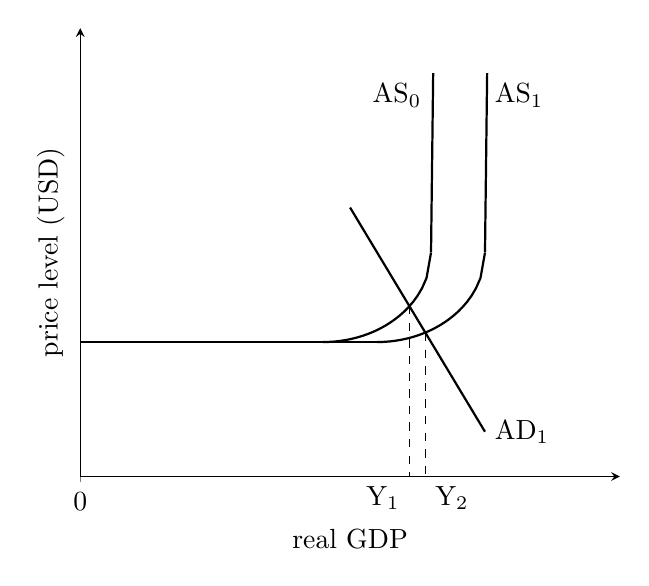
\begin{tikzpicture}[scale=1]
      \begin{axis}[
          axis lines=left,
          xlabel={real GDP},
          ylabel={price level (USD)},
          xmin=0, xmax=1,
          ymin=0, ymax=1,
          xtick={0}, ytick={\empty},
          clip=false
        ]

        \addplot[thick, domain=0:0.55] {0.3};
        \addplot[thick, domain=0.55:0.75] {0.5 - sqrt(1/25 - (x-0.55)^2)};
        \addplot[thick, domain=0.75:0.754] {100*x - 74.5};
        \node[right] at (0.75, 0.85) {AS$_1$};

        \addplot[thick, domain=0.45:0.65] {0.5 - sqrt(1/25 - (x-0.45)^2)};
        \addplot[thick, domain=0.65:0.654] {100*x - 64.5};
        \node[left] at (0.65, 0.85) {AS$_0$};

        \addplot[thick, domain=0.5:0.75] {1.6-2*x};
        \node[right] at (0.75, 0.1) {AD$_1$};


        \draw[dashed] (0.61, 0.38) -- (0.61, 0);
        \node[below left] at (0.61, 0) {Y$_1$};

        \draw[dashed] (0.64, 0.32) -- (0.64, 0);
        \node[below right] at (0.64, 0) {Y$_2$};

      \end{axis}
    \end{tikzpicture}
    \caption{Increase in AS}
  \end{center}
\end{wrapfigure}
\noindent Next, the new creation of 17,000 jobs will increase potential output, which equates to long term economic growth.
Specifically, the effect of these new jobs can potentially be manifest as a decrease in the natural rate of employment, corresponding to an increase in labor as a factor of production.
Consequently, with more production of key commodities such as aluminium, steel, cement, batteries and solar panels, the amount of output supplied at any given price level is increased.
In other words, the Mozambican economy experiences an increase in aggregate supply thanks to this increase in jobs.
Thus, it is a form of long-term growth and aligns with the incentive of the government, so the \textbf{intervention} is justified.

This is illustrated in \textbf{Figure 2}, with AS$_0$ and AD$_1$ still the same, and AS$_1$ corresponding to the increased aggregate supply following this change.
As the figure shows, it is now possible to create a higher amount of real output without significantly increasing the price level.
Additionally, the actual real GDP is also increased, from Y$_1$ to Y$_2$, aligning with the reported data on the GDP of Mozambique.

Finally, and most pertinently in regards to \textbf{intervention} is the aspects of supply management present in this policy.
The choice to dedicate the funds mainly on industry, transport, communications, and services, all of which related to infrastructure, is a form of interventionist supply management.
The action of the government imposing improvements in infrastructure increases efficiency in production, resulting in higher demand.

Similarly, the establishment of 'Green Energy Mozambique' is the government's \textbf{intervention} to support sustainable production, thus accounting as market-based supply management.
The benefit lies in slowing down pollution and the depletion of natural resources, which allows the economy to produce equally efficiently in the future.

These factors also work to increase the aggregate supply as in \textbf{Figure 2}, while the possibility to export a portion of the commodities produced in this industrial park increases aggregate demand as in \textbf{Figure 1}.
All these improvements combined means it is reasonable to expect more economic growth in Mozambique in the future, if climate shocks and political tensions can be successfully avoided.

%NOTES:
% Distinguish G and I clearly
% Logical ordering: read the book
%  The new jobs are CREATED by the development in infrastructure
%  differentiate short/long run changes more clearly
%  Labor market diagram maybe?
% Diagram labels/captions.

\end{document}